\chapter{Data Collection}

Being from Russia and having graduated with a bachelor degree in linguistics in Moscow, I have been a part of multiple projects related to studying minority languages in Russia. My experience showed that there is a lot of effort in Russian linguistic community towards creating resources for those languages. \todo{maybe move up to the introduction}

There are 93 indigenous minority languages spoken in Russia according to Ethnologue (\parencite{lewis2009ethnologue}; the number should not be seen as precise because of the language vs.\ dialect uncertainty). 78 of these languages are written and over the half of those are prominently represented on the Internet. Some of these languages have Wikipedia articles, blogs and twitter accounts written entirely in their language. The languages belong to different families, but their written orthography, with the exception of a handful of Finnic languages, is based on Cyrillic alphabet. Note, that it does not mean that they all have the same alphabet

While many of these languages are largely represented on the Web, they still remain under-resourced. The majority of the languages used in this thesis for language identification have never been tried for this task before.

With the large amount of research in linguistics and NLP being done with the text resources published online, we need to be able to identify the languages of smaller languages in Russia in order to be able to collect substantial amount of data in those languages to conduct linguistic research.


\section{Data sources}

The data collection for this work is largely relying on the data provided by a project by students at the School of Linguistics at National Research University Higher School of Economics that were creating minority languages corpora as part of their master theses.\footnote{\url{http://web-corpora.net/wsgi3/minorlangs/about}} I did not use their ready-to-use corpora, but crawled the links referencing web-pages in particular languages using the crawlers developed within the same project. As they do not have a name I will refer to their project as \textit{Minorlangs}, as the link of their website suggests. 

\textit{Minorlangs} provides a variaty of different resources to collect a corpus, mainly being urls of particular pages, websites of domains that are likely to be written entirely in the minority language (so, not only the text from that url has to be extracted, but all the texts from the links on that page refer to and all the links that those pages refer to on the same website, etc.), as well as the links of webpages from various social media, such as Facebook,\footnote{\url{facebook.com}} Twitter,\footnote{\url{twitter.com}}, a question answering website ASKfm\footnote{\url{ask.fm}}, Russian biggest social media website Vkontakte\footnote{\url{vk.com}} and other.

\todo[inline]{Add a table with distribution of the resources and a few words about it}

\section{Data collection methods}
To collect the websites \textit{Minorlangs} uses Yandex.XML tool, which allows users to receive the responses to searches in Yandex\footnote{yandex.ru}, the most used search engine in Russia.

The authors have manually compiled a list of lexical markers unique to particular minority languages, i.e.\ most common function words that are unique for this particular language and do not contain diacritic or character that do not appear on the Russian keyboard (as they are often omitted or changed in writing).

Then based on those markers up to 1000 requests per day could be made (the limit set by the service). Certain links were ignored, i.e.\ known websites with the info about the languages, websites with scientific texts that may include research on minority languages, music and video websites, containing only names of the songs or videos but not full texts, as well as Wikipedia pages. For full description of the system's architecture see (CITE\todo{cite})


I rely on the \textit{Minorlang} project to have used the truly unique markers to identify the websites in particular languages. While I do clear out pages and posts written entirely in Russian, I assume that there is no mix-up between the other languages.

Using the links and a crawler that extracts texts from the pages (provided by the project as well) I extract the data in minority languages from the websites. This data however cannot be used straight away. The crawler collects a lot of meta-information (e.g.\ mark-up of the pages), such as the dates of the blog posts and navigation links between different parts of the websites. As most of the blogs and news resources are hosted on the Russian websites and do not have that information translated. In order to exclude those uses I exclude the lines that are less than 4 words long from the dataset.

\section{Filtering Russian out}
The long contact with Russian language was bound to influence the minority languages on the territory of Russian Federation. My experience of working with some of these languages (see i.e.\ \cite{clif}) showed that they are prone to loan a lot of words from Russian. A lot of words do not have an equivalent in the smaller language, and some are just very common code-switches. However, the websites that I am crawling also contain a lot of texts entirely in Russian, sometimes due to the mistakes of the request responses and sometimes just because people write (and comment) in different languages on the same website. Note that the vast majority of speakers of minority languages are bilingual, as well as literate in both languages. It is save to assume that people who speak the minority languages also fluently speak Russian (even with large efforts to save minority languages in Russia, the education is still provided primarily in Russian). 
Of course keeping the texts in Russian will only reduce the accuracy of the language identification system by mixing up the labels and introducing noise, but filtering out Russian words completely would also be counter-intuitive and would make the data less representative of the real language usage. \textit{Minorlangs} also removes tokens in English (including names of the companies and websites) and emojis. I feel that this information should be kept to preserve the authenticity of the data. I do, however, remove the lines written entirely in Arabic, which is common on the predominantly Muslim territories.

\textit{Minorlangs} identifies the languages with character trigram model of Russian language and uses it on the word level, thus excluding instances of all Russian words (using not the most reliable approach), while as I mentioned before, languages of Russia are largely influenced by Russian and have a significant number of loan words from Russian, which do not always adopt the smaller language morphology (to distinguish with a trigram model) and should definitely be considered part of the language. Thus, I used a much more simplified model. When extracting data, I my system splits it into sentences with an nltk sentence tokenizer (CITE\todo{cite something}) and then splits those sentences into tokens with an nltk tokenizer\todo{talk about the tokenizers}, removes the punctuation marks and lowers the register\todo{is this a correct word in English?}. The words from the sentence are then compared to the unigram list consisting the entire corpus of multi-domain corpus of Russian language,  OpenCorpora\footnote{\url{http://opencorpora.org/}} (164465 unique tokens). If more than the half of the words in the sentence are in the list, the sentence is considered in Russian and is thrown out, otherwise the sentence is treated as belonging to the minority language. This way I can keep longer code-switches without introducing too much noise to the data. The sentences are then added to file, with the label and the url that they came from.\footnote{The data is available MAKE A REPO WITH DATA ASK ABOUT COPYRIGHTS}
Overall, 2145666 sentences have eliminated due to overwhelming amount of Russian words.

\section{Cross-domain data}

\textit{Minorlangs} also provides the links for downloading the data from Russian social media website Vkontakte for 41 out of 47 languages above. I have crawled that data as well, but have not used it as part of the main data I am training the system on. This data is used to determine the influence of increased training data from a different domain as well as cross-domain testing. We report on the results further in this work. \todo {make a reference to results section} 
\todo[inline]{I have not actually downloaded it yet. It does not work, sent an email to the 'project' email, did not get a response yet. I they won't soon, I'll email their supervisor, he used to be my professor. Should be easy to fix, it is just missing a config file, I am sure someone must have it. Add to the table later + write a few sentences in the overview}

\section{Overview of the collected data} \todo{A full page report. Talk about how the speakers don't correspond to the presence online}


\todo[inline]{Do not have a full written text for an overview yet. SHould I do it at all. It is not related to the project directly, but it is interesting. The minorlangs website provides their own statistics on the amount of links they collected, but as half of them don't work anymore, I fell like the lines and tokens vs. number of speakers is more interesting.\\ This is the data after filtering out Russian.\\ Should I add the vk.com data (when I have it) as 2 additional columns?\\
The f-scores (word unigram model) will not be in this table. It is only here to see whether the size matters. and the results are quite interesting.\\ Should I Northern Yukaghir because it is too tiny and only ruins everything?
}

This work is aimed at developing tools for low-resourced languages, and investigating the (lower) limits of data needed for successful language identification, I did not concentrate as much on collecting as much data as possible. Instead I have only used the data from separate urls (and not the entire domains) and Vkontakte data. You can see the overview of the collected data in the Table (REFERENCE\todo{reference. Keep here or as an appendix?}). The table is sorted by the number of sentences collected per language.

\resizebox{\textwidth}{!}{
\begin{tabular}{|p{4cm}|l|p{1.3cm}|r|r|r|r|r|} 
\hline

lang & lang family & native speakers & id & lines & tokens & &f1\\
\hline
\hline
Tatar   & Turkic &	4280000 &  tat & 416428 & 4208681 &  & 0.92 \\
Chechen    & Nakho-Dagestanian & 1354705 &  che & 201007 & 1863447 &  & 0.91 \\
Bashkir    & Turkic & 1150000 & bak & 125134 & 1170574 &  & 0.92 \\
Kabardian  & Abkhazo-Adyghean  & 515672 &  kbd & 102305 & 885434  &  & 0.88 \\
Buryat    & Mongolic & 283000 &  bxr & 101286 & 987638  &  & 0.88 \\
Chuvash    & Turkic &	1152404 &  chv & 86599  & 637411  &  & 0.83 \\
Eastern \& Meadow Mari    &  Uralic & 365316 &  mhr & 82981  & 700941  &  & 0.89 \\
Yakut    & Turkic & 450140 &  sah & 82836  & 727122  &  & 0.82 \\
Ingush    & Nakho-Dagestanian &305868 &  inh & 55123  & 512757  &  & 0.71 \\
Erzya    & Uralic & 431692 &  myv & 52984  & 372254  &  & 0.82 \\
Komi-Zyrian    & Uralic & 160599 &  kpv & 48947  & 352996  &  & 0.73 \\
Udmurt    & Uralic & 324338 &  udm & 47574  & 404315  &  & 0.81 \\
Tuvinian    & Turkic & 253673 &  tyv & 46509  & 343603  &  & 0.83 \\
Lezghian    & Nakho-Dagestanian & 	402173 &  lez & 43710  & 343389  &  & 0.91 \\
Southern Altai & Turkic   & 55720 &  alt & 32298  & 239846  &  & 0.94 \\
Karachay-Balkar  & Turkic  & 305364 &   krc & 27705  & 186895  &  & 0.85 \\
Nogai   & Turkic & 	88328 &  nog & 26805  & 344323  &  & 0.85 \\
Avar & Nakho-Dagestanian    & 715297  &   ava & 26478  & 153654  &  & 0.86 \\
Adyghe & Abkhazo-Adyghean   & 117489 &   ady & 24426  & 204491  &  & 0.71 \\
Evenki  & Tungusic  & 	4800 &  evn & 23999  & 381639  &  & 0.86 \\
Gilyak  & isolate  & 	198 &  niv & 22642  & 244880  &  & 0.66 \\
Lak  & Nakho-Dagestanian  & 145895 &  lbe & 17214  & 108980  &  & 0.93 \\
Moksha & Uralic   &  2025 &   mdf & 15163  & 165356  &  & 0.69 \\
Khakas  & Turkic  & 42604 &  kjh & 13545  & 158186  &  & 0.93 \\
Kalmyk  & Mongolic  & 	80546 &  xal & 12549  & 94406   &  & 0.83 \\
Komi-Permyak & Uralic  & 	63106 &  koi & 9972   & 53919   &  & 0.65 \\
Nanai  & Tungusic  & 1347 &  gld & 9058   & 57540   &  & 0.75 \\
Chukot  & Chukotko-Kamchatkan  & 5095 &  ckt & 6292   & 48756   &  & 0.66 \\
Nenets & Uralic   & 21926 &  yrk & 5698   & 42505   &  & 0.77 \\
Shor & Turkic   & 2839 &  cjs & 3237   & 20962   &  & 0.81 \\
Tabassaran & Nakho-Dagestanian    & 	126136 &  tab & 3182   & 16766   &  & 0.52 \\
Kumyk  & Turkic  & 	426212 &   kum & 2879   & 19522   &  & 0.52 \\
Udi  & Nakho-Dagestanian  & 2266 &  udi & 2798   & 19823   &  & 0.85 \\
Abaza & Abkhazo-Adyghean   &  37831   &   abq & 1893   & 13527   &  & 0.68 \\
Muslim Tat & Indo-European   & 26000* &  ttt & 1531   & 25404   &  & 0.91 \\
Dargwa & Nakho-Dagestanian   & 	42000 &  dar & 1183   & 7928    &  & 0.74 \\
Tsakhur & Nakho-Dagestanian   & 	10596 &  tkr & 1111   & 7126    &  & 0.53 \\
Southern Yukaghir  & Uralic  & 50 &  yux & 1101   & 7531    &  & 0.82 \\
Koryak & Chukotko-Kamchatkan   & 1665 &  kpy & 1002   & 5819    &  & 0.72 \\
Kubachi & Nakho-Dagestanian   & 3400 & dar2 & 721    & 9825    &  & 0.52 \\
Karagas  & Turkic  & 	93 &  kim & 651    & 4173    &  & 0.84 \\
Mansi & Uralic   & 938 &  mns & 584    & 3415    &  & 0.45 \\
Archi & Nakho-Dagestanian    & 970 &   aqc & 152    & 1769    &  & 0.22 \\
Rutul & Nakho-Dagestanian    & 30360 &  rut & 139    & 1618    &  & 0.82 \\
Khanty & Uralic   &  9584 &  kca & 113    & 984     &  & 0.78 \\
Even  & Tungusic  & 	5656 &  eve & 86     & 809     &  & 0.69 \\
Northern Yukaghir  & Uralic  & 30-150 &  ykg & 34     & 245     &  & 0.22 \\
\hline
\end{tabular}}

%coverage
\todo{add map as an appendix}
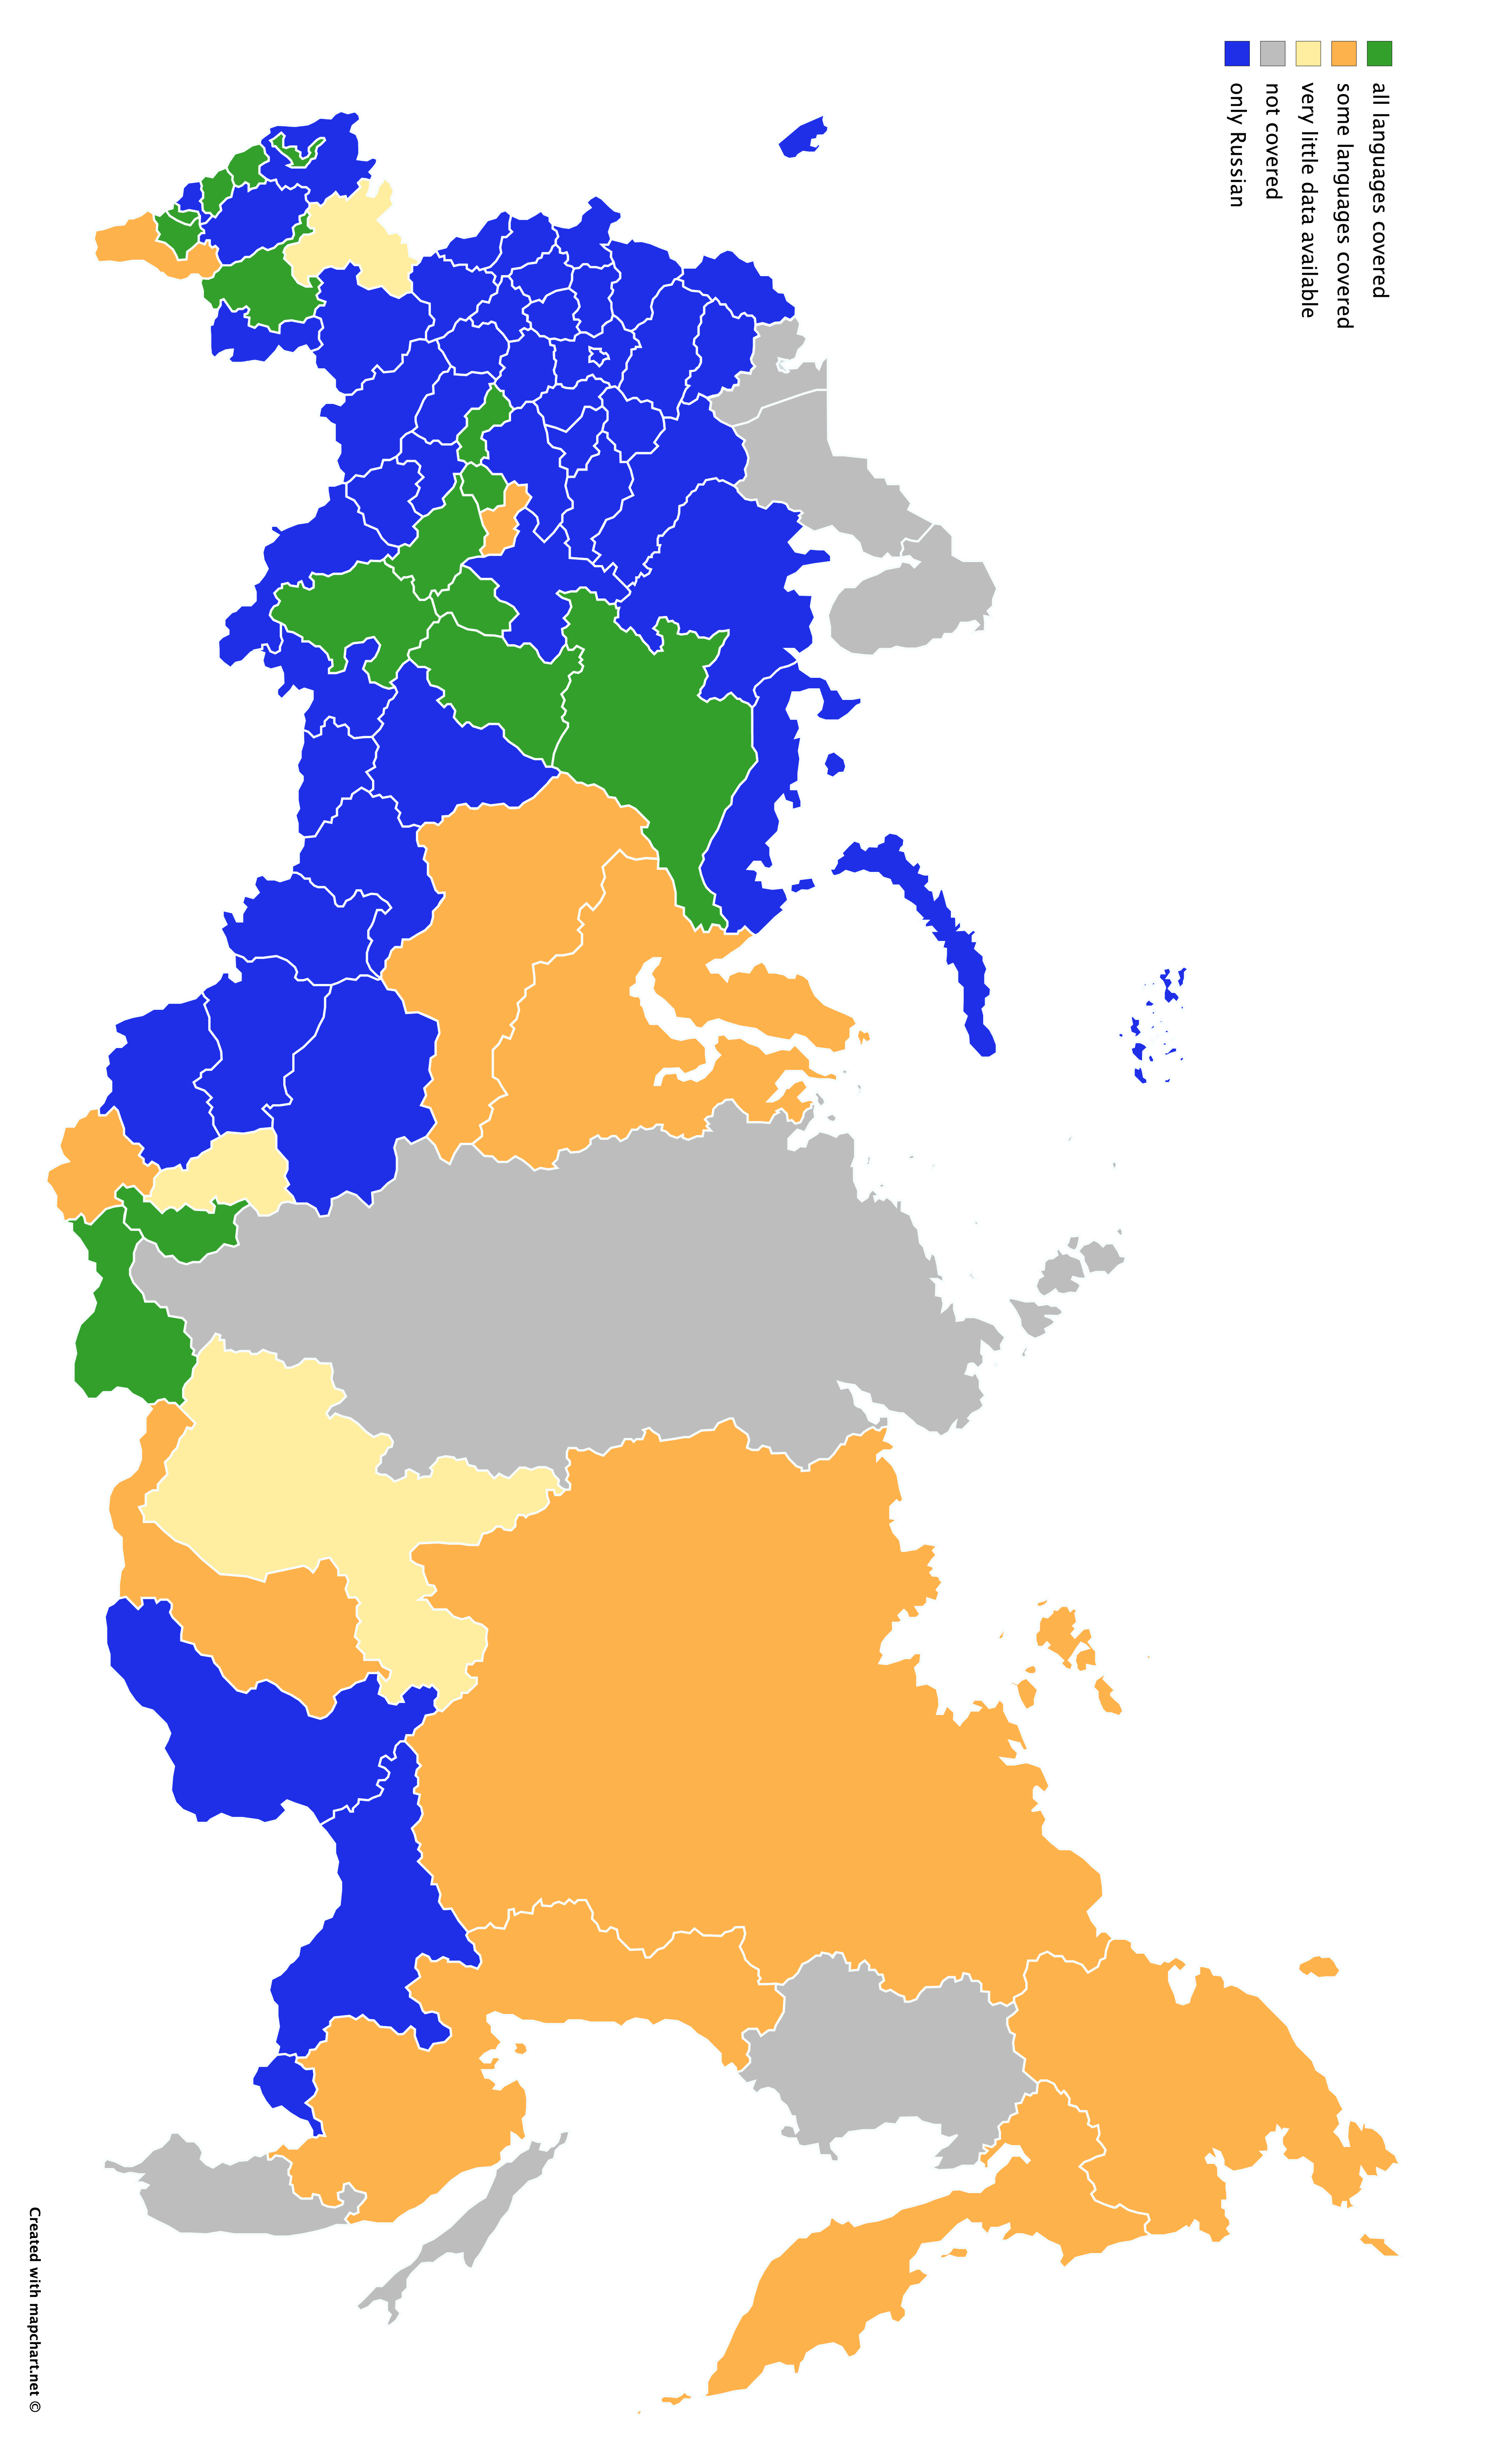
\includegraphics[width=0.9\textwidth]{language_map_russia}

% \begin{itemize}
%     \item Why do we want to work with languages of Russia
%     \item What are the languages of Russia (families, places), talk about influence of Russian
%     \item What kind of languages we can access
%     \item A map
%     \item Data collection methods
%     \item Different domains (mainly, Wikipedia, VK \& Facebook, blogs, twitter, other) \& why we want to have a cross-domain language identification system. Talk about the assumptions that the language should not be too different. Make estimations of sizes of different domain for different languages. Which ones can we use for cross-domain training/testing?
% \end{itemize}

% In short, the goal of the project would be to create a language identification system that would not need a dictionary for language identification, as to be able to be trainable for under-resourced languages.

% As some of the languages might not have much data, the aim will be to build the most generalized system possible, so that the accuracy for the out-of-domain data would not drop much.

%  I am planning to use Wikipedia as a primary resource of data for the languages of Russia. Even though some minority languages are not largely represented and there is noise in the form of articles in the majority languages of the region where they are spoken, many of them can still be used for language identification. The articles in the wrong language can often be dismissed by their length: the longer the article the more likely it is to be in the right language. Only sentences with the correct alphabet for the language will be used. A threshold for the amount of Russian words can also be set.
 
% The tweets (in order to have more domains to train and test on) can be found on the basis of the Wikipedia lexicon. As most of these languages have been in a long contact with Russian we can eliminate its lexicon by using words from big monolingual corpora which do not overlap with Russian corpus, then search for the tweets that contain those words and take all the tweets by the user. Some of these tweets may contain code-switching and thus, should be eliminated from the training. They can however be used for the testing; in that case the algorithm for word-level code-switching annotation developed in my bachelor's thesis can be used. %\todo{would be cool to cite yourself with your BA thesis here :P} 


% As I hope that a finer-grained system could work well on code-mixed texts as well, I will need to collect multilingual data for testing. There is data collected for EMNLP workshops of 2014 and 2016, some of tweets collected for the monolingual corpus will also be bound to contain code-switching. I would also like to try modeling texts/tweets with code-switching, using twitter and parallel corpora, such as was done in \textcite{vrl2010multilingual}, where they combined shorter tweets in different languages into longer multilingual ones. Possibly some blogs will also be available.

%Collect tweets from epicenters of language use, if the language contains symbols that are not part of Russian alphabet, take the rest of the tweets by the user. Otherwise use dictionary to locate user tweeting in a language and then using all of their tweets, checking with dictionary and/or alphabet for the majority to be in the language.

%\begin{tabular}{|r|r|} 
%\hline
%mns & 393634 \\
%aqc & 206 \\
%ttt & 19186 \\
%tyv & 2238254 \\
%
%ckt & 230716 \\
%
%ykg & 867 \\
%
%koi & 132821 \\
%
%cjs & 29622 \\
%
%yux & 6309 \\
%
%myv & 583650 \\
%
%tkr & 10016 \\
%
%dar & 2632497 \\
%
%itl & 107 \\
%
%mdf & 228437 \\
%
%kbd & 1978395 \\
%
%nog & 591255 \\
%
%tab & 16572 \\
%
%che & 6448622 \\
%
%evn & 324432 \\
%
%kum & 223781 \\
%
%mhr & 3365212 \\
%
%ady & 232056 \\
%
%alt & 293572 \\
%
%inh & 616943 \\
%
%chv & 15676435 \\
%
%krc & 699233 \\
%
%rut & 1812 \\
%
%xal & 989829 \\
%
%gld & 63197 \\
%
%kas & 10188 \\
%
%niv & 179954 \\
%
%kpv & 872851 \\
%
%lez & 1065773 \\
%
%yrk & 87240 \\
%
%ava & 978896 \\
%
%udi & 20960 \\
%
%bxr & 3767431 \\
%
%lbe & 1632921 \\
%
%kim & 8401 \\
%
%rts & 2 \\
%
%abq & 124098 \\
%
%kpy & 58947 \\
%\hline
%\end{tabular}

% \begin{table}[!ht]
%     \centering
%     \begin{tabular}{|p{3.5cm}|p{7.5cm}|} 
%     \hline
%     Monolingual data & \vspace{-2\topsep}\begin{itemize}\setlength\itemsep{-.25em}
%         \item Wikipedias of languages of Russia
%         \item Tweets of the same languages
%         \item Existing corpora of languages of Russia (see \url{http://web-corpora.net/?l=en})
%         \item Data used for the other systems:
%         \vspace{-\topsep}\begin{itemize}\setlength\itemsep{-.25em}
%             \item \parencite{vrl2014accurate} -- 97 languages, 1M messages
%             \item \parencite{lui2011cross} -- 97 languages
%             \item \parencite{bergsma2012language} -- 65 languages, 10M messages
%             \item DSL 2014
%             \item DSL 2015
%             \item DSL 2016
%             \item DSL 2017
%         \end{itemize}\vspace{-\topsep}
%     \end{itemize}\vspace{-2\topsep}\\
%     \hline
%     Multilingual data & \vspace{-2\topsep}\begin{itemize}\setlength\itemsep{-.25em}
%         \item EMNLP workshop 2014 + 2016
%         \item ALTA-2010 Shared Task
%         \item Artificial tweets
%         \item Blogs
%     \end{itemize}\vspace{-2.5\topsep}\\
%     \hline
%     \end{tabular}
%     \caption{Overview of available data.}
%     % \label{tab:my_label}
% \end{table}%\todo{caption? And maybe also itemize in the right column for clarity}





